\chapter{Implementación de la solución de lado del servidor}\label{servidor}
Como se comentó en el final del capítulo anterior, se ha hecho uso de una página web básica en un servidor Linux contratado y configurado desde cero (puertos a utilizar, frameworks, actualizaciones, entre otros). Esto con el fin de poder ir realizando pruebas y al mismo tiempo tener un espacio preparado para el backend de la aplicación. 

En este capítulo se ahondará en su adquisición y características generales.

\section{Requerimientos}
Desde un inicio se tuvo en cuenta la necesidad de tener conexión a un servidor capaz de ofrecer el almacenamiento de datos, procesamiento de los mismos y despliegue de ellos a los profesionales de la salud. Es por ello que en un inicio se hizo búsqueda de una página web con dichas características. Pero, rápidamente se hace necesario distinguir los servicios ofrecidos para el desarrollo de backend con acceso universal (dirección ip pública).

\subsection{Tipos de alojamiento Web}
El hosting\cite{hosting_web} (alojamiento web en español) consiste en un servicio prestado a través de internet, por el cual se permite el almacenamiento (a través del uso de un servidor) de distintos contenidos en la web.

\newpage
Para comprender a cabalidad de qué trata, es necesaria una distinción y definición previa de la palabra servidor en nuestro contexto: Se pueden definir dos grandes formas de servidor, uno físico y uno informático (comúnmente llamado servidor web).
Por una parte, el servidor físico provee de recursos electrónicos como lo puede ser: Capacidad de memoria ram, disco duro, procesamiento, entre otros. Por otro lado, el servidor "informático" es aquel \textbf{programa} con la capacidad de procesar peticiones web y opcionalmente (habitual) responderlas.

En los últimos años, el mercado de este tipo de servicios ha ido en aumento y por tanto se han generado distintas alternativas de obtenerlo. Existiendo más de una docena de formatos distintos con los cuales se ofrece, pero en este apartado solo veremos los más relevantes para el proyecto (dejando de lado servicios específicos como el de correos electrónicos, entre otros).

\begin{enumerate}
	\item \textbf{Alojamiento compartido:}
	En este alojamiento se permite compartir un mismo servidor físico entre distintos clientes y sus páginas web. Entre sus ventajas está el corto periodo de tiempo para la puesta en marcha y el costo, aunque entre sus principales desventajas se encuentra el rendimiento general, la poca flexibilidad de configuración y la disminución en seguridad y estabilidad.
	\item \textbf{Servidor virtual (VPS):}
	Servicio en el cual se comparten los recursos de hardware, pero se aíslan las distintas instancias a través de máquinas virtuales. Entre sus ventajas está el control completo del sistema al ofrecer comúnmente una base solo de sistema operativo, programas base y dirección IP pública. Su principal desventaja es un bajo rendimiento bajo alta carga.
	\item \textbf{Servidor dedicado:}
	Alojamiento en el cual se emplea una computadora con todos sus recursos al servicio de un único cliente, permitiendo tercerizar el cuidado de la máquina y la conexión a internet de la misma. Entre sus principales ventajas está el control casi absoluto del servicio a configurar y el alto rendimiento al no compartir el hardware. Su principal desventaja es el costo asociado a este servicio tan personalizado.
	\item \textbf{Alojamiento en la nube:}
	Basado en las tecnologías más innovadoras, permite el uso de múltiples máquinas actuar como un sistema unificado. Dotando así de gran capacidad de expansión (crecimiento en tiempo real). Su principal desventaja al igual que el anterior, es su alto costo.
\end{enumerate}

Como se puede observar entre las opciones disponibles, existen diferencias tanto a nivel técnico como económico que hacen necesario un análisis más específico de los requerimientos del proyecto.

\subsection{Requerimientos del proyecto}

El proyecto requiere de una serie de características a nivel de Backend, entre las que destacan:


\begin{enumerate}[]\centering
	\item \textbf{Bajo costo}
	\item \textbf{Alta flexibilidad}
	\item \textbf{Alto rendimiento}
\end{enumerate}

Al estar en una etapa de desarrollo se considera irrelevante la capacidad de cómputo y de ancho de banda ofrecido. Así y considerando las opciones de la anterior sección se destaca la opción de un alojamiento de tipo VPS, con el cual poder acceder a una máquina virtual con todas las prestaciones de un sistema operativo (como lo es acceso a socket e instalación manual de herramientas).

\newpage
\section{Hosting VPS}

A partir de los requerimientos del proyecto se hace notoria la posible falta de rendimiento al escoger el alojamiento VPS, es por esto que al momento de gestionar el contrato con una prestadora de servicio se priorizó aquellas que tuvieran almacenamiento SSD (Disco en estado sólo en español), aumentando así notoriamente el rendimiento de la máquina virtual. Además, seleccionar un proveedor local del servicio tanto por temas de soporte, como por el tiempo de respuesta en las peticiones hechas desde el mismo territorio nacional. Además de lo anterior, se destaca la necesidad de un servidor con la opción de manejar los puertos del equipo y no solo el 80 (destinado a peticiones web).

De esta forma se logra acceder a una máquina con las siguientes características:
\textbf{Empresa:} OpenCloud en Chile por \$6.000 pesos mensuales.\\ 
\textbf{IP:} xxx.xxx.xxx.xxx\\
\textbf{Ubicación:} Chile.\\
\textbf{Ancho de banda:} 60 [Mb/s]\\
\textbf{Tráfico:} 2 [TB] (Bajada + Subida) mensuales.\\
\textbf{Sistema Operativo:} Ubuntu v16.04 - 64 bit\\
\textbf{Procesador:} Monoprocesador a 2.2 [GHz]\\
\textbf{Ram:} 2 [GB]\\
\textbf{Disco Duro:} 20 [GB]\\
\newpage
En una primera instancia se maneja comunicación síncrona a través de peticiones HTTP comunes y experimentación con WebSocket (detallado más adelante).
Proporciona un canal de comunicación bidireccional y full-duplex sobre un único socket TCP, permitiendo una comunicación entre el servidor y el navegador.
Cada 100 [ms] se envía desde el navegador una marca de tiempo correspondiente al último dato recibido. Esta marca no corresponde al último dato existente, se envía una actualización de la cantidad de datos y el último dato actual, además de la nueva marca de tiempo.

A través de una petición GET se entregan los datos a ingresar:\\ \textit{http://galenoproject.sytes.net/data/?name=ECG\&data=8\&save=yes}

En el ejemplo anterior se agregará un documento a la base de datos con los parámetros name y data, el parámetro save es utilizado para controlar si se debe o no almacenar dichos datos.

Luego, a partir de la dirección: \textit{http://galenoproject.sytes.net/} se puede observar:

\begin{figure}[H]
	\centering
	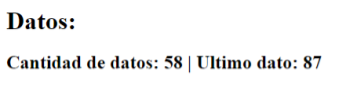
\includegraphics[scale=0.6]{figuras/servidor/primera_version.png}
	\caption{Primera versión de la página web. Fuente: Elaboración propia}
	\label{first_example}
\end{figure}

El contenido de la figura \ref{first_example} corresponde a la cantidad de datos actual en la base de datos y el último dato recibido. 

En las siguientes secciones se detalla la configuración del equipo y las herramientas empleadas hasta el momento.

\newpage
\section{Servidor Tornado}
Framework de desarrollo web basado en Python, ofrece alto rendimiento, gran escalabilidad y ofrece hasta 10.000 usuarios conectados bajo conexiones continuas gracias a su tratamiento asincrónico de las entradas y salidas del sistema. Utilizado para procesar solicitudes como entrada o salida de datos.

\textbf{Implementado:} Python v2.7.12, Tornado v4.5.1

\section{MongoDB}
Base de datos no relacional destacada por su escalabilidad, rendimiento y gran disponibilidad. Utilizado para almacenar los datos recopilados y su posterior lectura.

\textbf{Implementado:} MongoDB v3.2.13

\section{Nginx}
Servidor Web/Proxy Inverso de alto rendimiento. Utilizado para redirigir de forma interna peticiones entrantes a distintos servidores que se están comunicando en distintos puertos de forma interna.

\textbf{Implementado:} Nginx v1.10.0

\section{DNS No-IP}
Compañía que provee DNS dinámicos por pago o gratuitos con ciertas limitantes, como lo pueden ser las alternativas de dominios disponibles. Utilizado para enmascarar la ip pública del hosting y acceder a través de un nombre de dominio.

\textbf{Implementado:} galenoproject.sytes.net


